% Options for packages loaded elsewhere
% Options for packages loaded elsewhere
\PassOptionsToPackage{unicode}{hyperref}
\PassOptionsToPackage{hyphens}{url}
\PassOptionsToPackage{dvipsnames,svgnames,x11names}{xcolor}
%
\documentclass[
  letterpaper,
  DIV=11,
  numbers=noendperiod]{scrartcl}
\usepackage{xcolor}
\usepackage[margin=1in]{geometry}
\usepackage{amsmath,amssymb}
\setcounter{secnumdepth}{5}
\usepackage{iftex}
\ifPDFTeX
  \usepackage[T1]{fontenc}
  \usepackage[utf8]{inputenc}
  \usepackage{textcomp} % provide euro and other symbols
\else % if luatex or xetex
  \usepackage{unicode-math} % this also loads fontspec
  \defaultfontfeatures{Scale=MatchLowercase}
  \defaultfontfeatures[\rmfamily]{Ligatures=TeX,Scale=1}
\fi
\usepackage{lmodern}
\ifPDFTeX\else
  % xetex/luatex font selection
  \setmainfont[]{DejaVu Serif}
  \setmonofont[]{DejaVu Sans Mono}
\fi
% Use upquote if available, for straight quotes in verbatim environments
\IfFileExists{upquote.sty}{\usepackage{upquote}}{}
\IfFileExists{microtype.sty}{% use microtype if available
  \usepackage[]{microtype}
  \UseMicrotypeSet[protrusion]{basicmath} % disable protrusion for tt fonts
}{}
\makeatletter
\@ifundefined{KOMAClassName}{% if non-KOMA class
  \IfFileExists{parskip.sty}{%
    \usepackage{parskip}
  }{% else
    \setlength{\parindent}{0pt}
    \setlength{\parskip}{6pt plus 2pt minus 1pt}}
}{% if KOMA class
  \KOMAoptions{parskip=half}}
\makeatother
% Make \paragraph and \subparagraph free-standing
\makeatletter
\ifx\paragraph\undefined\else
  \let\oldparagraph\paragraph
  \renewcommand{\paragraph}{
    \@ifstar
      \xxxParagraphStar
      \xxxParagraphNoStar
  }
  \newcommand{\xxxParagraphStar}[1]{\oldparagraph*{#1}\mbox{}}
  \newcommand{\xxxParagraphNoStar}[1]{\oldparagraph{#1}\mbox{}}
\fi
\ifx\subparagraph\undefined\else
  \let\oldsubparagraph\subparagraph
  \renewcommand{\subparagraph}{
    \@ifstar
      \xxxSubParagraphStar
      \xxxSubParagraphNoStar
  }
  \newcommand{\xxxSubParagraphStar}[1]{\oldsubparagraph*{#1}\mbox{}}
  \newcommand{\xxxSubParagraphNoStar}[1]{\oldsubparagraph{#1}\mbox{}}
\fi
\makeatother


\usepackage{longtable,booktabs,array}
\newcounter{none} % for unnumbered tables
\usepackage{calc} % for calculating minipage widths
% Correct order of tables after \paragraph or \subparagraph
\usepackage{etoolbox}
\makeatletter
\patchcmd\longtable{\par}{\if@noskipsec\mbox{}\fi\par}{}{}
\makeatother
% Allow footnotes in longtable head/foot
\IfFileExists{footnotehyper.sty}{\usepackage{footnotehyper}}{\usepackage{footnote}}
\makesavenoteenv{longtable}
\usepackage{graphicx}
\makeatletter
\newsavebox\pandoc@box
\newcommand*\pandocbounded[1]{% scales image to fit in text height/width
  \sbox\pandoc@box{#1}%
  \Gscale@div\@tempa{\textheight}{\dimexpr\ht\pandoc@box+\dp\pandoc@box\relax}%
  \Gscale@div\@tempb{\linewidth}{\wd\pandoc@box}%
  \ifdim\@tempb\p@<\@tempa\p@\let\@tempa\@tempb\fi% select the smaller of both
  \ifdim\@tempa\p@<\p@\scalebox{\@tempa}{\usebox\pandoc@box}%
  \else\usebox{\pandoc@box}%
  \fi%
}
% Set default figure placement to htbp
\def\fps@figure{htbp}
\makeatother





\setlength{\emergencystretch}{3em} % prevent overfull lines

\providecommand{\tightlist}{%
  \setlength{\itemsep}{0pt}\setlength{\parskip}{0pt}}



 


\KOMAoption{captions}{tableheading}
\makeatletter
\@ifpackageloaded{tcolorbox}{}{\usepackage[skins,breakable]{tcolorbox}}
\@ifpackageloaded{fontawesome5}{}{\usepackage{fontawesome5}}
\definecolor{quarto-callout-color}{HTML}{909090}
\definecolor{quarto-callout-note-color}{HTML}{0758E5}
\definecolor{quarto-callout-important-color}{HTML}{CC1914}
\definecolor{quarto-callout-warning-color}{HTML}{EB9113}
\definecolor{quarto-callout-tip-color}{HTML}{00A047}
\definecolor{quarto-callout-caution-color}{HTML}{FC5300}
\definecolor{quarto-callout-color-frame}{HTML}{acacac}
\definecolor{quarto-callout-note-color-frame}{HTML}{4582ec}
\definecolor{quarto-callout-important-color-frame}{HTML}{d9534f}
\definecolor{quarto-callout-warning-color-frame}{HTML}{f0ad4e}
\definecolor{quarto-callout-tip-color-frame}{HTML}{02b875}
\definecolor{quarto-callout-caution-color-frame}{HTML}{fd7e14}
\makeatother
\makeatletter
\@ifpackageloaded{caption}{}{\usepackage{caption}}
\AtBeginDocument{%
\ifdefined\contentsname
  \renewcommand*\contentsname{Table of contents}
\else
  \newcommand\contentsname{Table of contents}
\fi
\ifdefined\listfigurename
  \renewcommand*\listfigurename{List of Figures}
\else
  \newcommand\listfigurename{List of Figures}
\fi
\ifdefined\listtablename
  \renewcommand*\listtablename{List of Tables}
\else
  \newcommand\listtablename{List of Tables}
\fi
\ifdefined\figurename
  \renewcommand*\figurename{Figure}
\else
  \newcommand\figurename{Figure}
\fi
\ifdefined\tablename
  \renewcommand*\tablename{Table}
\else
  \newcommand\tablename{Table}
\fi
}
\@ifpackageloaded{float}{}{\usepackage{float}}
\floatstyle{ruled}
\@ifundefined{c@chapter}{\newfloat{codelisting}{h}{lop}}{\newfloat{codelisting}{h}{lop}[chapter]}
\floatname{codelisting}{Listing}
\newcommand*\listoflistings{\listof{codelisting}{List of Listings}}
\makeatother
\makeatletter
\makeatother
\makeatletter
\@ifpackageloaded{caption}{}{\usepackage{caption}}
\@ifpackageloaded{subcaption}{}{\usepackage{subcaption}}
\makeatother
\usepackage{bookmark}
\IfFileExists{xurl.sty}{\usepackage{xurl}}{} % add URL line breaks if available
\urlstyle{same}
\hypersetup{
  pdftitle={Corpus Characterization},
  pdfauthor={Eric Rue; Rauf Agyemang},
  colorlinks=true,
  linkcolor={blue},
  filecolor={Maroon},
  citecolor={Blue},
  urlcolor={Blue},
  pdfcreator={LaTeX via pandoc}}


\title{Corpus Characterization}
\usepackage{etoolbox}
\makeatletter
\providecommand{\subtitle}[1]{% add subtitle to \maketitle
  \apptocmd{\@title}{\par {\large #1 \par}}{}{}
}
\makeatother
\subtitle{AlbertoChestnut/telugu-ocr --- Phase 1 Deliverable}
\author{Eric Rue \and Rauf Agyemang}
\date{2026-06-25}
\begin{document}
\maketitle

\renewcommand*\contentsname{Table of contents}
{
\setcounter{tocdepth}{3}
\tableofcontents
}

\providecommand{\teluguchars}[1]{#1}

\section{Abstract}\label{abstract}

This document characterizes the corpus used for a Telugu OCR pipeline
built as a class deliverable for CSCI/DASC 6020 (Summer 2026). Working
from the publicly available \texttt{AlbertoChestnut/telugu-ocr}
HuggingFace dataset, we developed against a five-book subset comprising
415 paired page images and ground-truth Unicode text files. We built an
inventory script that records per-page metadata (image dimensions, file
sizes, pairing integrity), computed corpus statistics, defined a
five-bucket quality taxonomy by structured visual inspection of a
stratified 97-page sample, and froze a stratified 30-page evaluation
subset (six pages per bucket) that all downstream phases score against.
The corpus is dominated by visually clean pages (approximately
two-thirds of the sample) with a long tail of skewed scans, complex
layouts, faded ink, and damaged pages that include scanning artifacts
and physical damage. These quality conditions directly determine the
preprocessing pipeline scope in Phase 2 and provide the per-bucket axis
along which model performance is reported in Phase 5.

\section{Introduction}\label{introduction}

The CSCI/DASC 6020 Summer 2026 class project asks teams to build an
end-to-end Telugu OCR pipeline using vision-capable large language
models, plus a validation framework that scores OCR quality without
depending on human ground truth. The project rubric is structured around
seven dimensions; this document addresses Dimension 1 (Corpus
Characterization and Problem Scoping). Subsequent documents and
deliverables address the remaining dimensions: preprocessing (Dimension
2), OCR pipeline and model comparison (Dimension 3), LLM-assisted
validation (Dimension 4), analysis (Dimension 5), code quality
(Dimension 6), and the final written report (Dimension 7).

Corpus characterization comes first in our sequence because every
downstream decision depends on understanding what kinds of pages the OCR
system has to handle. Preprocessing stage selection (deskew,
binarization, denoise, contrast enhancement) is justified by the visual
conditions actually present in the corpus. Model selection between
vision-capable LLMs and classical OCR is justified by per-bucket
performance expectations --- vision LLMs are expected to outperform
classical OCR specifically on the harder buckets (complex layout,
damaged pages). Sample size choices for evaluation are justified by the
corpus distribution. Without an explicit characterization phase,
downstream design decisions would rest on assumption rather than
evidence.

The document is structured as follows. We first describe the dataset's
provenance and our reasons for choosing it. We then describe the
methodology used to characterize the corpus --- inventory, statistics,
taxonomy, and stratified subset selection. Section ``Corpus Statistics''
presents the headline numerical findings. Section ``Quality Taxonomy''
defines five quality buckets and their inclusion criteria. Section
``Evaluation Subset'' describes the 30-page frozen evaluation set and
its rationale. Section ``Challenges and Implications for Preprocessing''
links each quality bucket to the preprocessing stage that targets it,
establishing the per-bucket hypotheses that Phase 5 tests. We close with
limitations and references.

\section{Dataset Provenance}\label{dataset-provenance}

We use the publicly available \texttt{AlbertoChestnut/telugu-ocr}
dataset hosted on HuggingFace Hub. The dataset consists of paired image
and text files: for every \texttt{.jpg} page scan there is a
corresponding \texttt{.txt} file containing Unicode-encoded Telugu text.
The dataset author collected approximately 221 books totalling roughly
13 GB of paired files; multiple other student teams in CSCI/DASC 6020
also converged on this dataset for their Phase 1 corpus, which we
mention here for transparency.

The instructor announced on 27 May 2026 that a course-provided corpus
would be delivered ``next week,'' but as of project start that corpus
had not been distributed and multiple teams' follow-up requests went
unanswered. We treated the schedule risk as binding and adopted
\texttt{AlbertoChestnut/telugu-ocr} rather than wait. Our final report's
methodology section discloses this choice and the alternative we did not
pursue.

The paired-file structure of \texttt{AlbertoChestnut/telugu-ocr} is
essential to our approach. The project specification asks teams to
``sample 30-50 pages across the quality spectrum and annotate them
manually'' to produce ground-truth text for evaluation. Because the
upstream dataset already ships paired images and ground-truth text, we
skip manual annotation entirely. Our work is to characterize and
stratify what we have, not to create new ground-truth.

For reproducibility, our download script pins the exact dataset revision
(commit \texttt{f2bd895b4932b648174a8f47066f4166469933a0}) so that both
team members and future readers can re-download the identical files. The
pinned revision is documented in \texttt{scripts/download\_dataset.py}.

\section{Methodology}\label{methodology}

Our corpus characterization proceeded in four sequential steps. Each
step produced an artifact consumed by the next.

\textbf{Step 1 --- Inventory.} A Python script walks the local dataset
directory, pairs each \texttt{.jpg} with its matching \texttt{.txt} file
by filename stem, extracts per-page metadata (image dimensions via
Pillow, file sizes from \texttt{stat}), and writes the result to
\texttt{data/external/corpus\_inventory.csv}. The script also verifies
the paired-file invariant (every \texttt{.jpg} has a matching
\texttt{.txt}) and runs an encoding spot-check on a small random sample
of text files to confirm UTF-8 NFC encoding. The inventory CSV becomes
the canonical ``table of contents'' for every downstream phase.

\textbf{Step 2 --- Statistics.} A Jupyter notebook loads the inventory
CSV and produces four distribution plots: image dimension scatter,
estimated DPI distribution, ground-truth text length distribution, and
image file-size distribution. The notebook also writes a small JSON file
(\texttt{data/external/corpus\_stats.json}) with headline numerical
findings used by the report and by downstream design decisions.

\textbf{Step 3 --- Quality taxonomy.} We define five quality buckets by
structured visual inspection. A stratified sample of 97 pages was
browsed page-by-page, observations were collected, and the observations
were clustered into five buckets with concrete, OCR-relevant inclusion
criteria. The buckets are documented in detail in the Quality Taxonomy
section below.

\textbf{Step 4 --- Stratified evaluation subset.} From the 97
hand-tagged pages we draw six pages per bucket (30 pages total) with a
fixed random seed, write the selection to
\texttt{data/external/eval\_subset.csv}, and copy the 30 image+text
pairs to \texttt{data/external/eval\_subset/}. This frozen subset is the
evaluation target for every Phase 3 OCR run, every Phase 4 CER/WER
computation, and every Phase 5 per-bucket analysis.

\textbf{Subset rather than full corpus.} We work with a five-book subset
(415 paired pages, approximately 190 MB) rather than the full 13 GB
corpus. The motivation is iteration speed: with 415 pages we can re-run
the inventory, the preprocessing pipeline, and the OCR adapters across
the full local set in minutes rather than hours, which matters in a
four-day delivery schedule. The five-book subset covers the file-size
and book-format variation observed in the full upstream listing, so we
expect it to be representative for the kinds of statistical and quality
claims this project makes. We disclose the subset choice in the
Limitations section.

\textbf{No manual annotation.} As stated in the previous section, we do
not annotate ground-truth text. The dataset's paired-file structure
provides it. Time we would otherwise spend on annotation goes to
building a stronger pipeline.

\section{Corpus Statistics}\label{corpus-statistics}

The 5-book subset comprises \textbf{415 paired pages} across \textbf{5
books}, drawn from the upstream \texttt{AlbertoChestnut/telugu-ocr}
HuggingFace dataset at the pinned commit. Per-book page counts:

{\def\LTcaptype{none} % do not increment counter
\begin{longtable}[]{@{}lr@{}}
\toprule\noalign{}
Book ID & Pages \\
\midrule\noalign{}
\endhead
\bottomrule\noalign{}
\endlastfoot
Kalidasa-Charitra\_by\_chilakamarthi\_lakshminarasimham & 133 \\
2015.385293.Paarijaata-Paharanamu & 110 \\
2015.389095.Shabhuka-Vadha & 75 \\
2015.328360.Andhra-Mahaniyulu & 60 \\
2030020025431\_-\_chitra\_leikhanamu & 37 \\
\textbf{Total} & \textbf{415} \\
\end{longtable}
}

Aggregate page-level statistics (from
\texttt{data/external/corpus\_stats.json}):

{\def\LTcaptype{none} % do not increment counter
\begin{longtable}[]{@{}ll@{}}
\toprule\noalign{}
Metric & Value \\
\midrule\noalign{}
\endhead
\bottomrule\noalign{}
\endlastfoot
Total books & 5 \\
Total pages & 415 \\
Median image width & 1500 pixels (uniform) \\
Median image height & 2261 pixels \\
Mean ground-truth text length & 3,145 chars \\
Median ground-truth text length & 2,882 chars \\
Median file size & 478 KB \\
DPI estimate (from typical 6-inch book width) & \textasciitilde250
DPI \\
\texttt{image\_width\_uniform} & \texttt{true} \\
\end{longtable}
}

\textbf{The image-width distribution is degenerate}: every image in the
subset is exactly 1500 pixels wide. We had originally planned to plot a
DPI histogram; with a single observed width, that collapses to a single
value (\textasciitilde250 DPI inferred from typical Telugu book physical
width). Rather than fake a histogram with a single bar, we report the
uniformity finding directly and set
\texttt{image\_width\_uniform:\ true} in the corpus stats JSON. The
Phase 2-5 pipeline does not depend on per-image DPI variation; this
finding is informational.

Headline distribution plots from
\texttt{notebooks/01\_corpus\_characterization.ipynb}:

\begin{figure}

\begin{minipage}[t]{\linewidth}

\begin{figure}[H]

{\centering 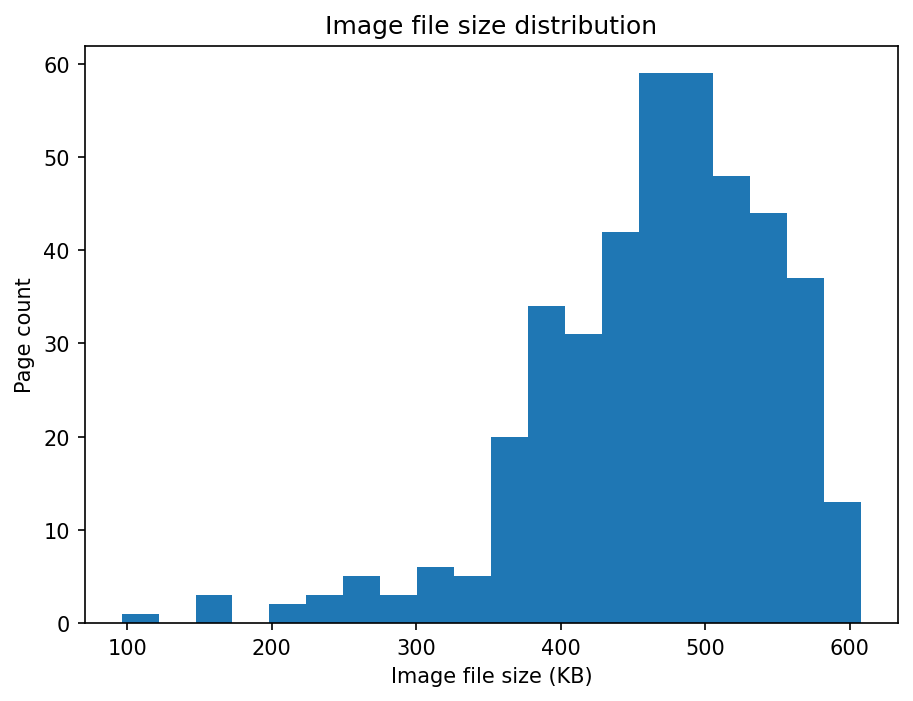
\includegraphics[width=0.85\linewidth,height=\textheight,keepaspectratio]{figures/corpus/file_size_distribution.png}

}

\subcaption{File-size distribution across the 5-book subset}

\end{figure}%

\end{minipage}%
\newline
\begin{minipage}[t]{\linewidth}

\begin{figure}[H]

{\centering 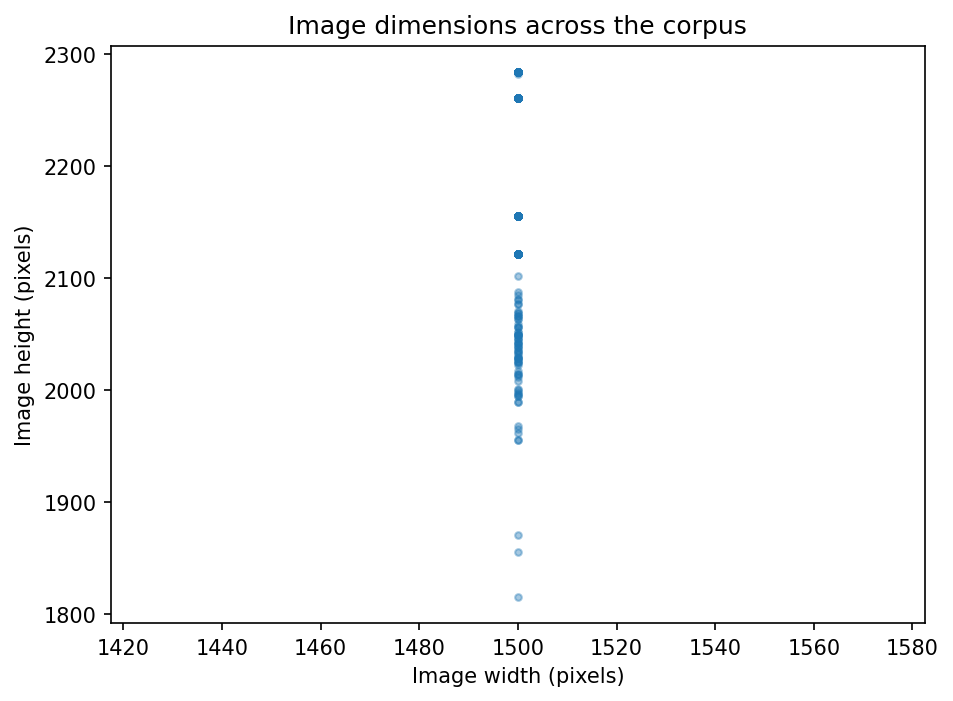
\includegraphics[width=0.85\linewidth,height=\textheight,keepaspectratio]{figures/corpus/image_dimensions_scatter.png}

}

\subcaption{Image-dimension scatter showing the uniform 1500-pixel
width}

\end{figure}%

\end{minipage}%
\newline
\begin{minipage}[t]{\linewidth}

\begin{figure}[H]

{\centering 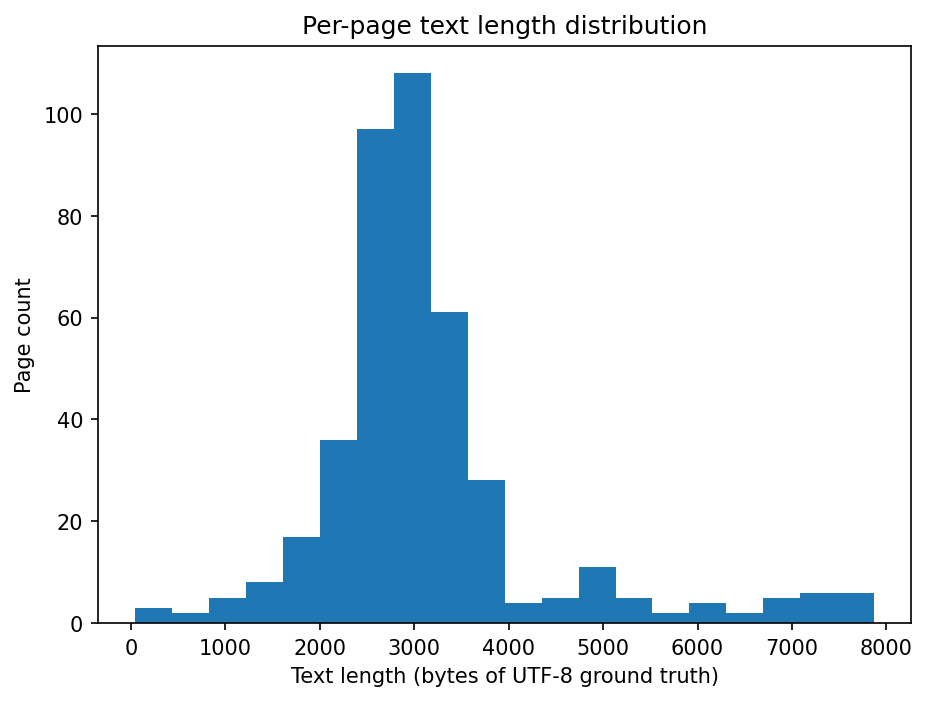
\includegraphics[width=0.85\linewidth,height=\textheight,keepaspectratio]{figures/corpus/text_length_distribution.png}

}

\subcaption{Per-page ground-truth text-length distribution}

\end{figure}%

\end{minipage}%

\end{figure}%

\section{Quality Taxonomy}\label{quality-taxonomy}

To make per-condition claims later in the project --- for example, ``our
OCR pipeline performs differently on pages with scanning artifacts
versus clean pages'' --- we partition the corpus into five quality
buckets. The buckets are defined by visual features observable directly
from the page image, without reading the Telugu text.

We arrived at these five buckets by a structured browsing pass. A
stratified sample of 47 pages (5 books × 5 image-file-size quintiles,
drawn with a fixed random seed for reproducibility) was reviewed page by
page and observations were collected. The observations were then
clustered into the five buckets below. Bucket definitions are
intentionally concrete --- they describe specific visual features rather
than impressionistic good-versus-bad judgments --- so a second annotator
should be able to apply them to a new page and reach the same bucket
approximately 80\% of the time.

When multiple features are present on a single page, the buckets are
applied with the following priority order (most severe first):

\begin{enumerate}
\def\labelenumi{\arabic{enumi}.}
\tightlist
\item
  \textbf{Damaged / Content Loss}
\item
  \textbf{Complex Layout}
\item
  \textbf{Faded}
\item
  \textbf{Skewed}
\item
  \textbf{Clean} (default)
\end{enumerate}

A page that is both skewed and damaged is assigned to Damaged. A page
that is both faded and has complex layout is assigned to Complex Layout.
The order reflects how strongly each feature dominates OCR difficulty.

\subsection{Clean}\label{clean}

\textbf{Definition.} Pages with crisp printed Telugu body text, the page
sitting square in the scan frame (no visible tilt), single-column layout
with no embedded illustrations or text-in-boxes, and no significant
scanning artifacts or fading. This is the default category --- pages go
here unless one of the other four buckets clearly applies.

\textbf{Inclusion criteria} (all must hold):

\begin{itemize}
\tightlist
\item
  Body-text characters are uniformly legible
\item
  Page tilt is visually undetectable (less than approximately 1 degree)
\item
  Layout is single-column flowing text
\item
  No drawings, illustrations, or text bounded in boxes or frames
\item
  No visible scanning artifacts (no white bands, no severe edge fading,
  no severe smudging)
\item
  No visible physical damage to the source page
\end{itemize}

\textbf{OCR relevance.} Baseline. The expected lower bound on CER (best
case) across the corpus comes from this bucket. Phase 5 reports
per-bucket CER so the Clean baseline is visible separately from harder
cases.

\begin{figure}[H]

{\centering 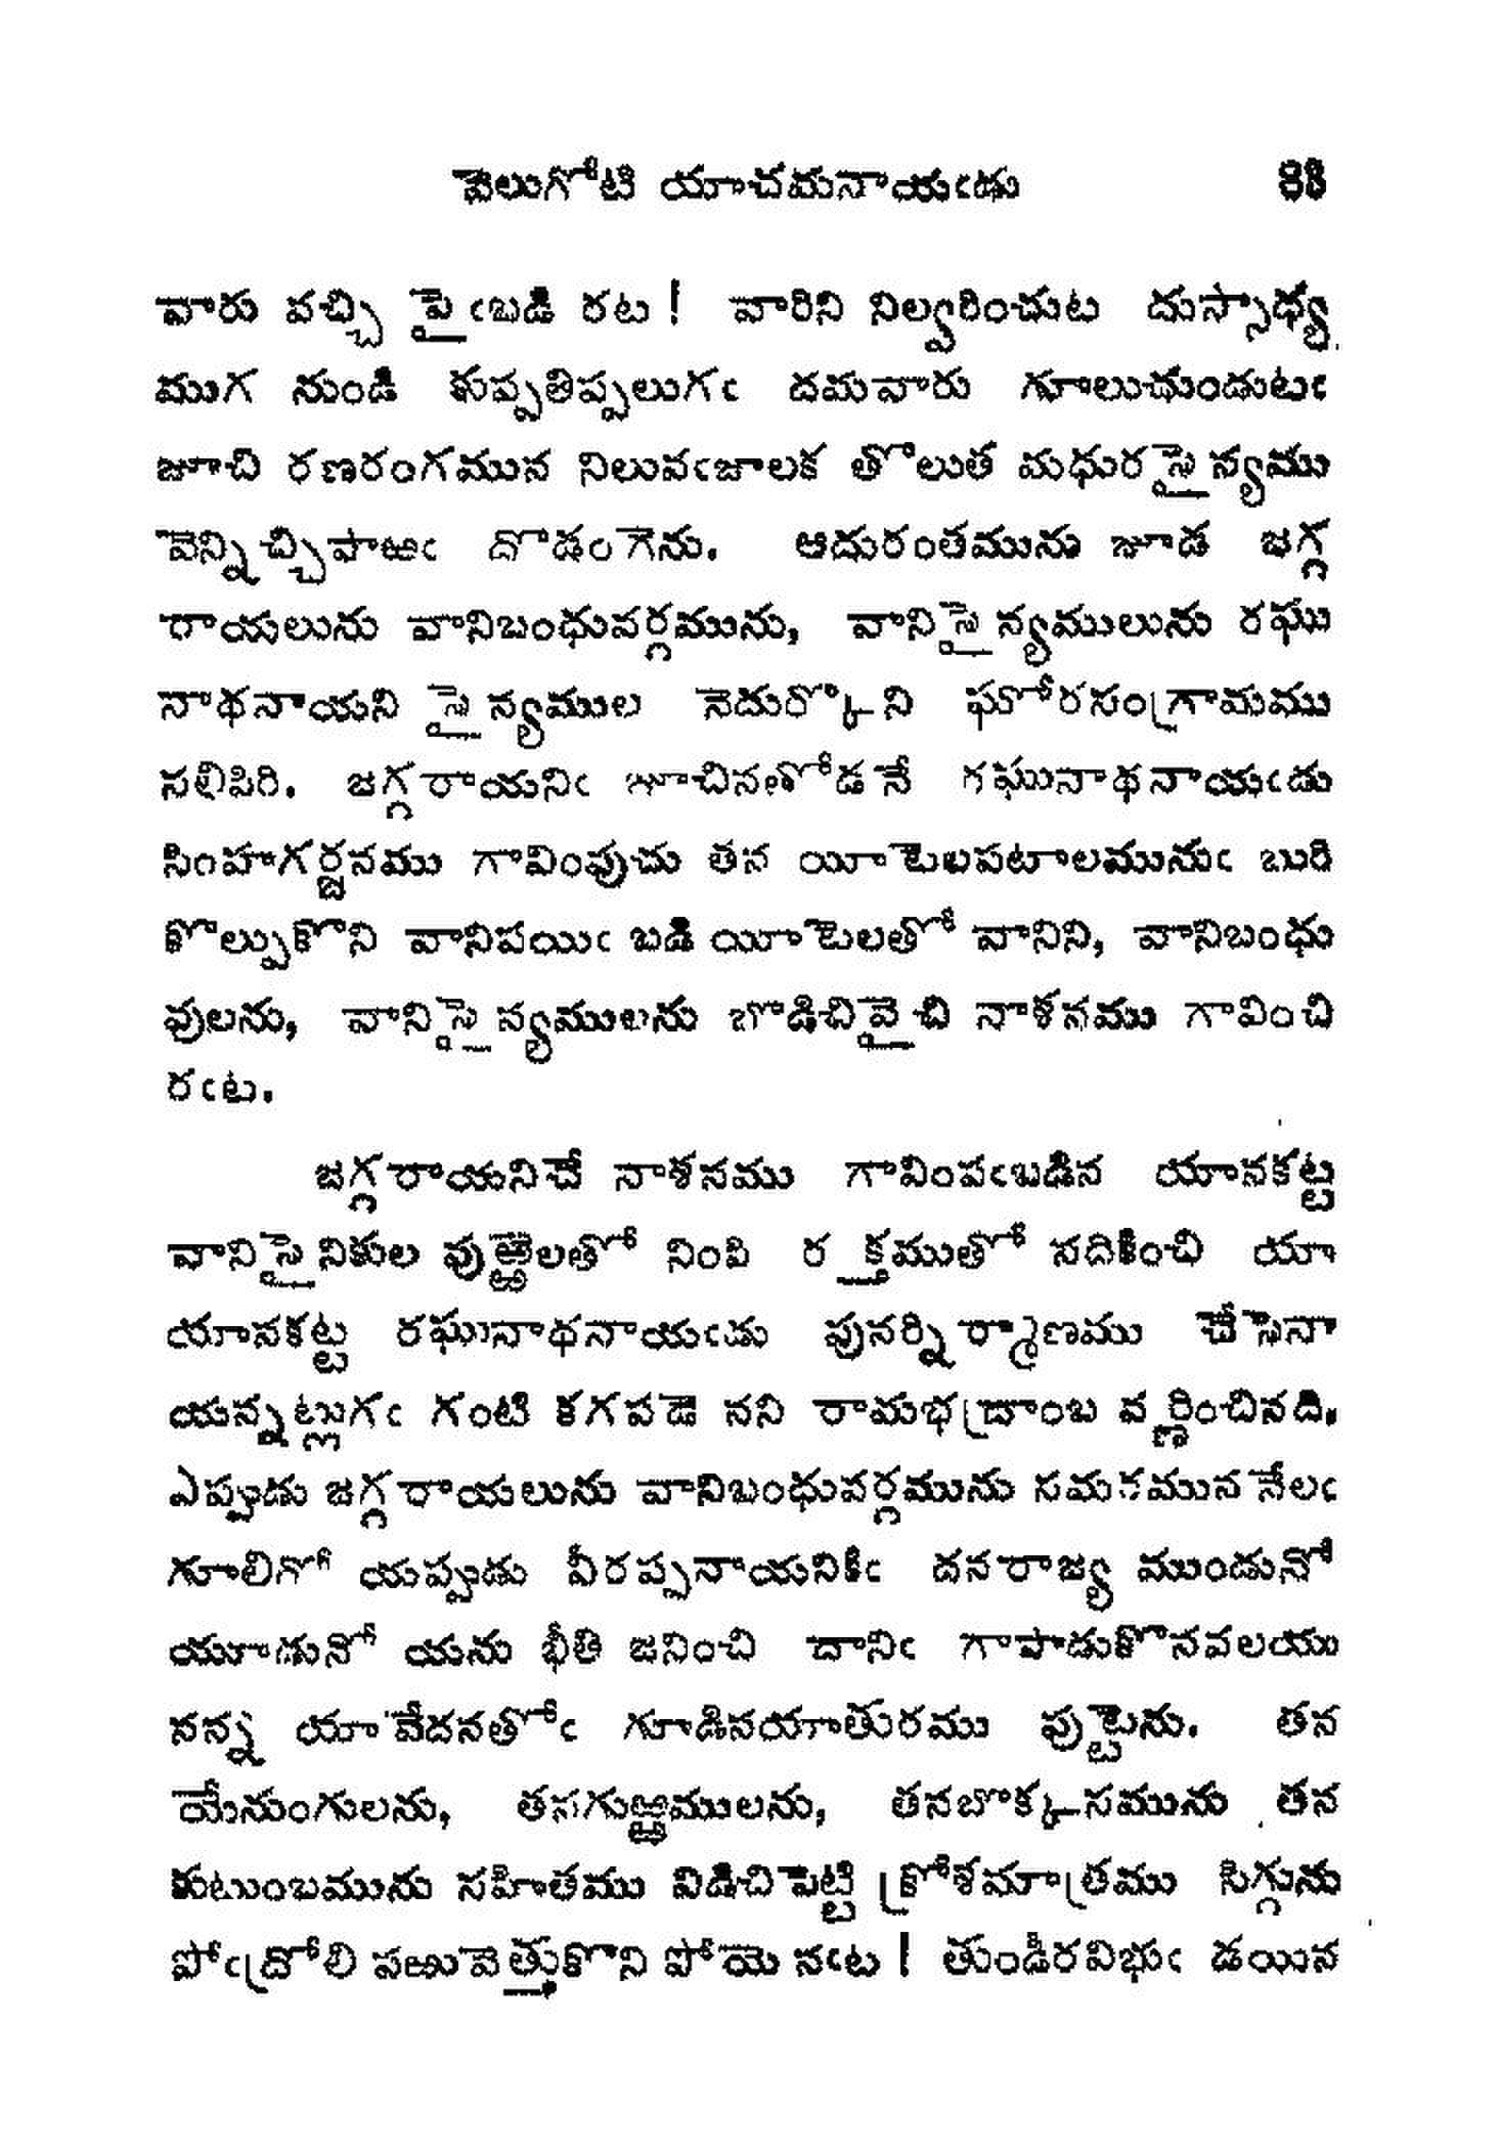
\includegraphics[width=0.6\linewidth,height=\textheight,keepaspectratio]{figures/corpus/quality_examples/clean.jpg}

}

\caption{Example: clean page.}

\end{figure}%

\subsection{Skewed}\label{skewed}

\textbf{Definition.} Pages where the printed content is visibly tilted
relative to the image frame, indicating the physical page was not
aligned square to the scanner glass when captured.

\textbf{Inclusion criteria} (all must hold):

\begin{itemize}
\tightlist
\item
  Body-text lines are clearly not horizontal --- a visible tilt is
  present
\item
  Tilt is at least approximately 2 degrees (visually unambiguous)
\item
  Text is otherwise legible --- not also faded, damaged, or in complex
  layout
\end{itemize}

\textbf{OCR relevance.} This is the bucket directly addressed by the
deskew preprocessing stage in Phase 2. We expect to observe a measurable
CER improvement on this bucket between the raw-OCR and preprocessed-OCR
runs in Phase 5.

\begin{figure}[H]

{\centering 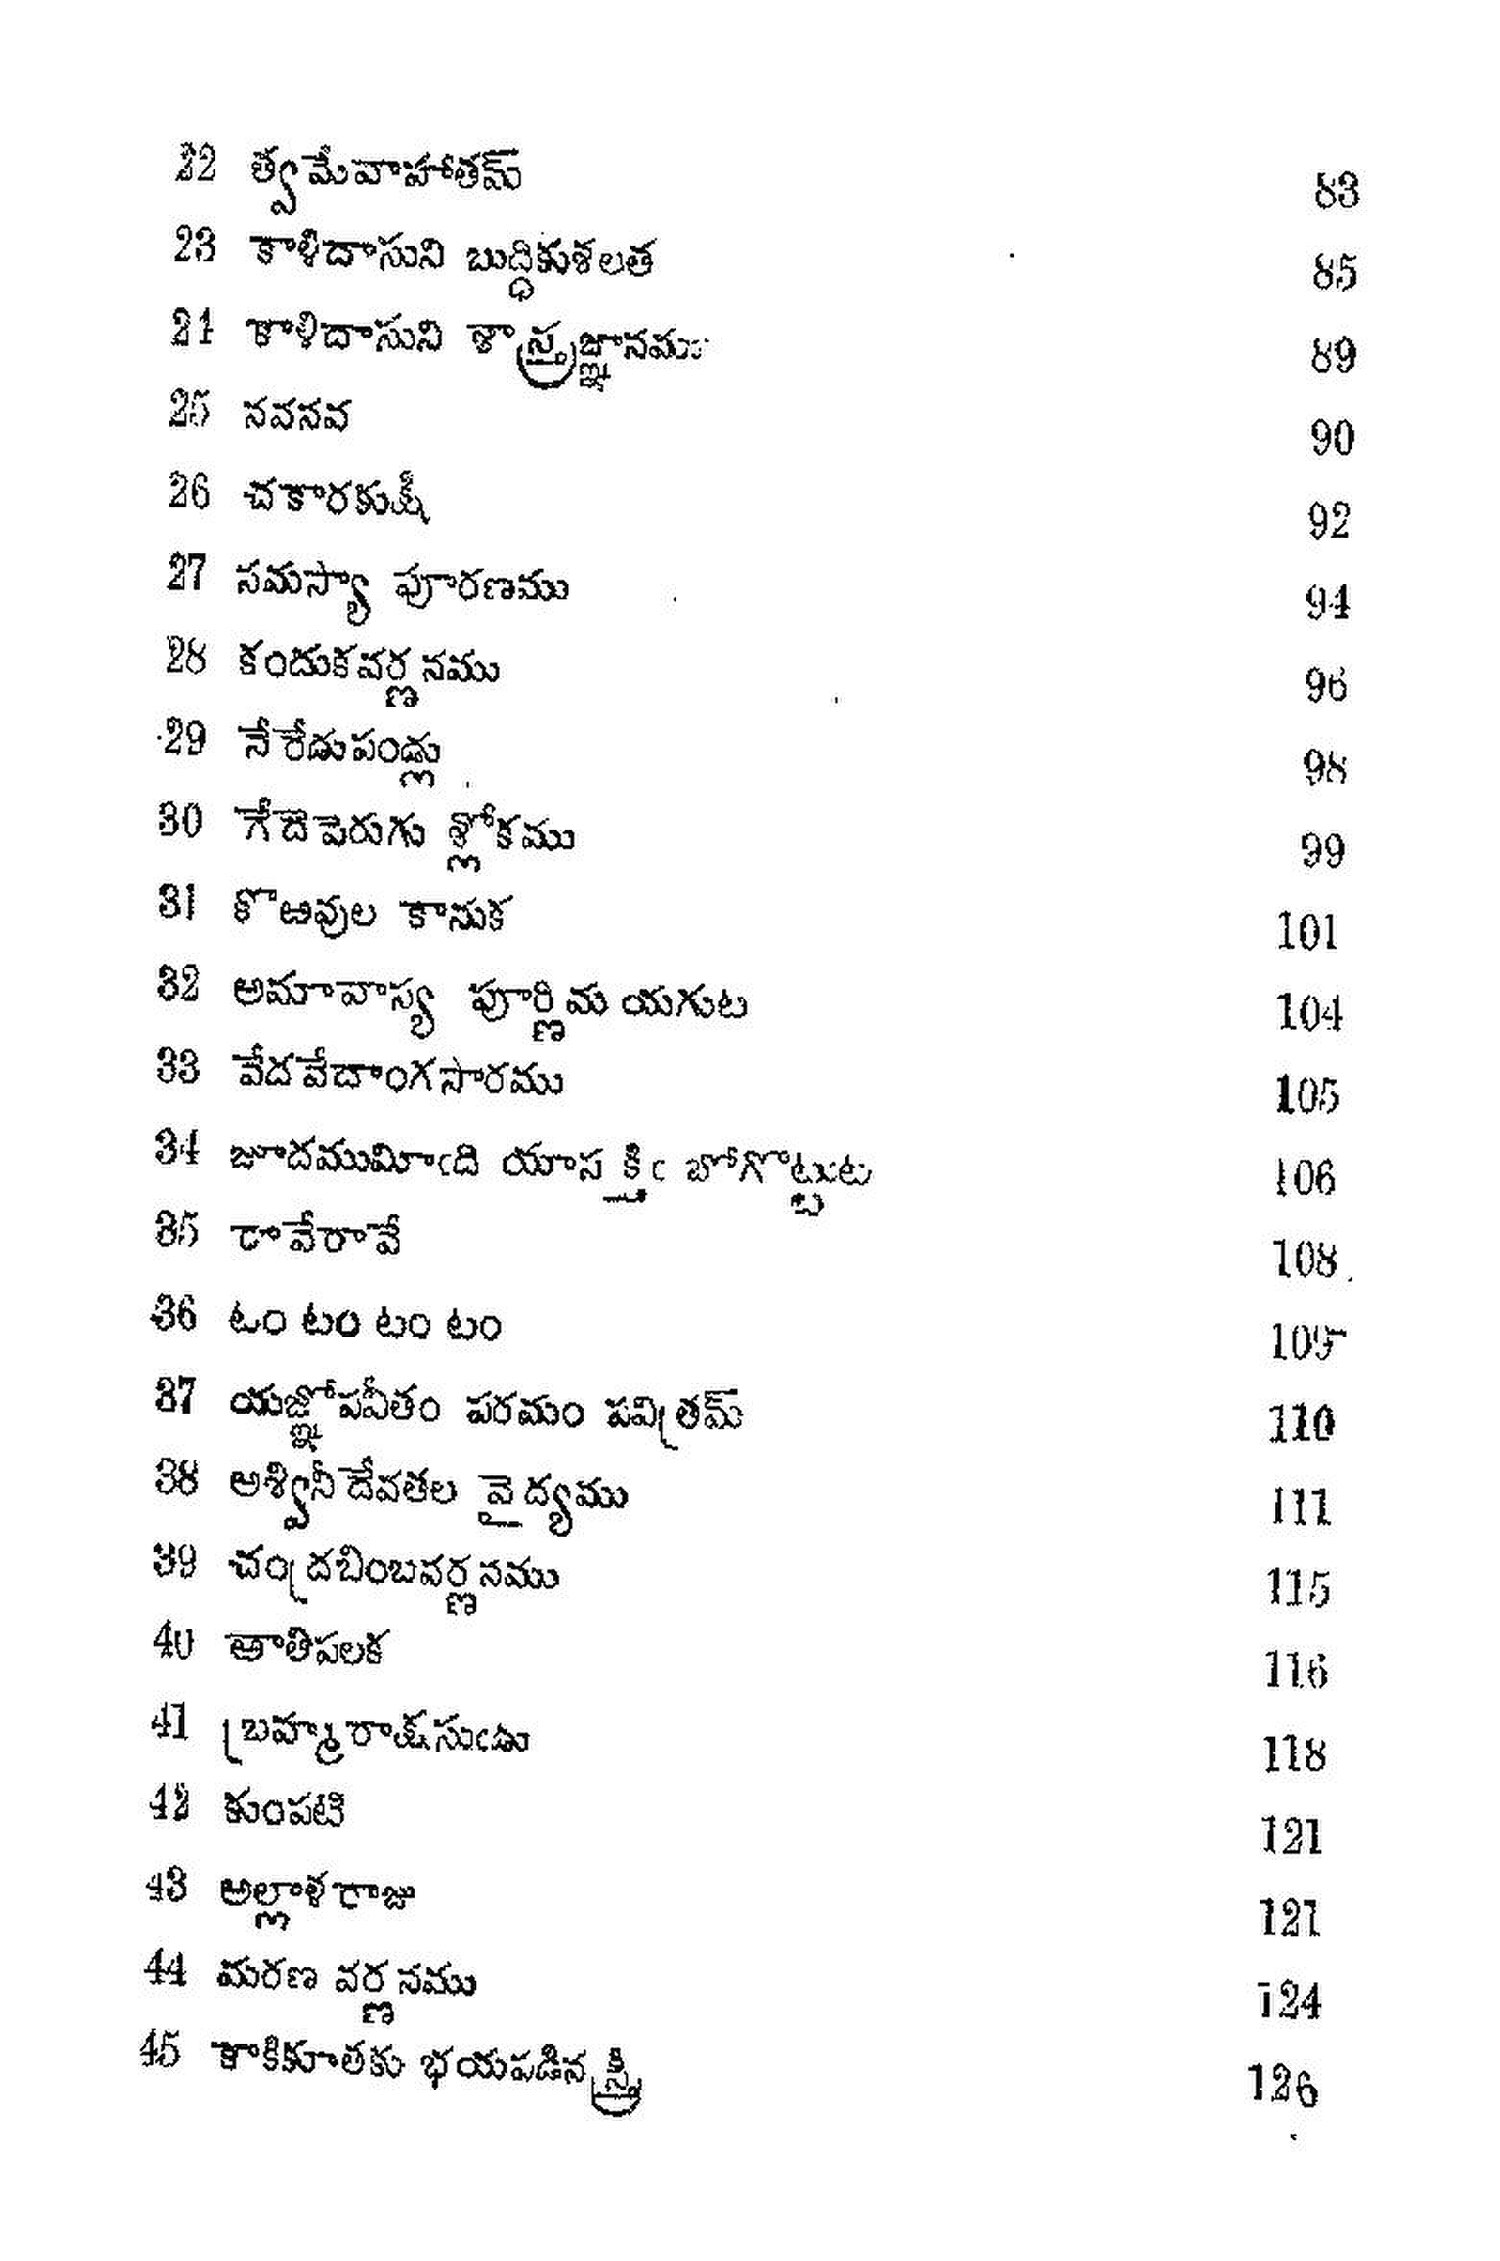
\includegraphics[width=0.6\linewidth,height=\textheight,keepaspectratio]{figures/corpus/quality_examples/skewed.jpg}

}

\caption{Example: skewed page.}

\end{figure}%

\subsection{Complex Layout}\label{complex-layout}

\textbf{Definition.} Pages where the structure deviates from
single-column flowing text. Includes pages with embedded illustrations,
text inside boxes or frames, multi-column layouts, tables, or pages
dominated by ornamental content rather than body text.

\textbf{Inclusion criteria} (any one is sufficient):

\begin{itemize}
\tightlist
\item
  Page contains at least one drawing or illustration covering
  approximately 10\% or more of the page area
\item
  Page contains text bounded in boxes, frames, or borders (not merely
  decorative dividers between paragraphs)
\item
  Page uses a multi-column body-text layout
\item
  Page contains tabular data
\item
  Page is dominated by visual or ornamental content rather than body
  text (for example, a title page)
\end{itemize}

\textbf{Disambiguation.} Normal Telugu typographic features such as
decorative section dividers (rows of stars or dots between paragraphs),
ornamental borders along the page edge, or numbered verses are NOT
sufficient on their own to place a page in Complex Layout. These are
standard features of Telugu publishing and appear throughout
otherwise-Clean pages.

\textbf{OCR relevance.} Vision-LLM OCR (Gemini) is expected to handle
complex layouts gracefully, whereas classical OCR (Tesseract) may
produce reading-order errors or skip non-text regions inconsistently.
This bucket is a key axis for the model-comparison story in Phase 5.

\begin{figure}[H]

{\centering 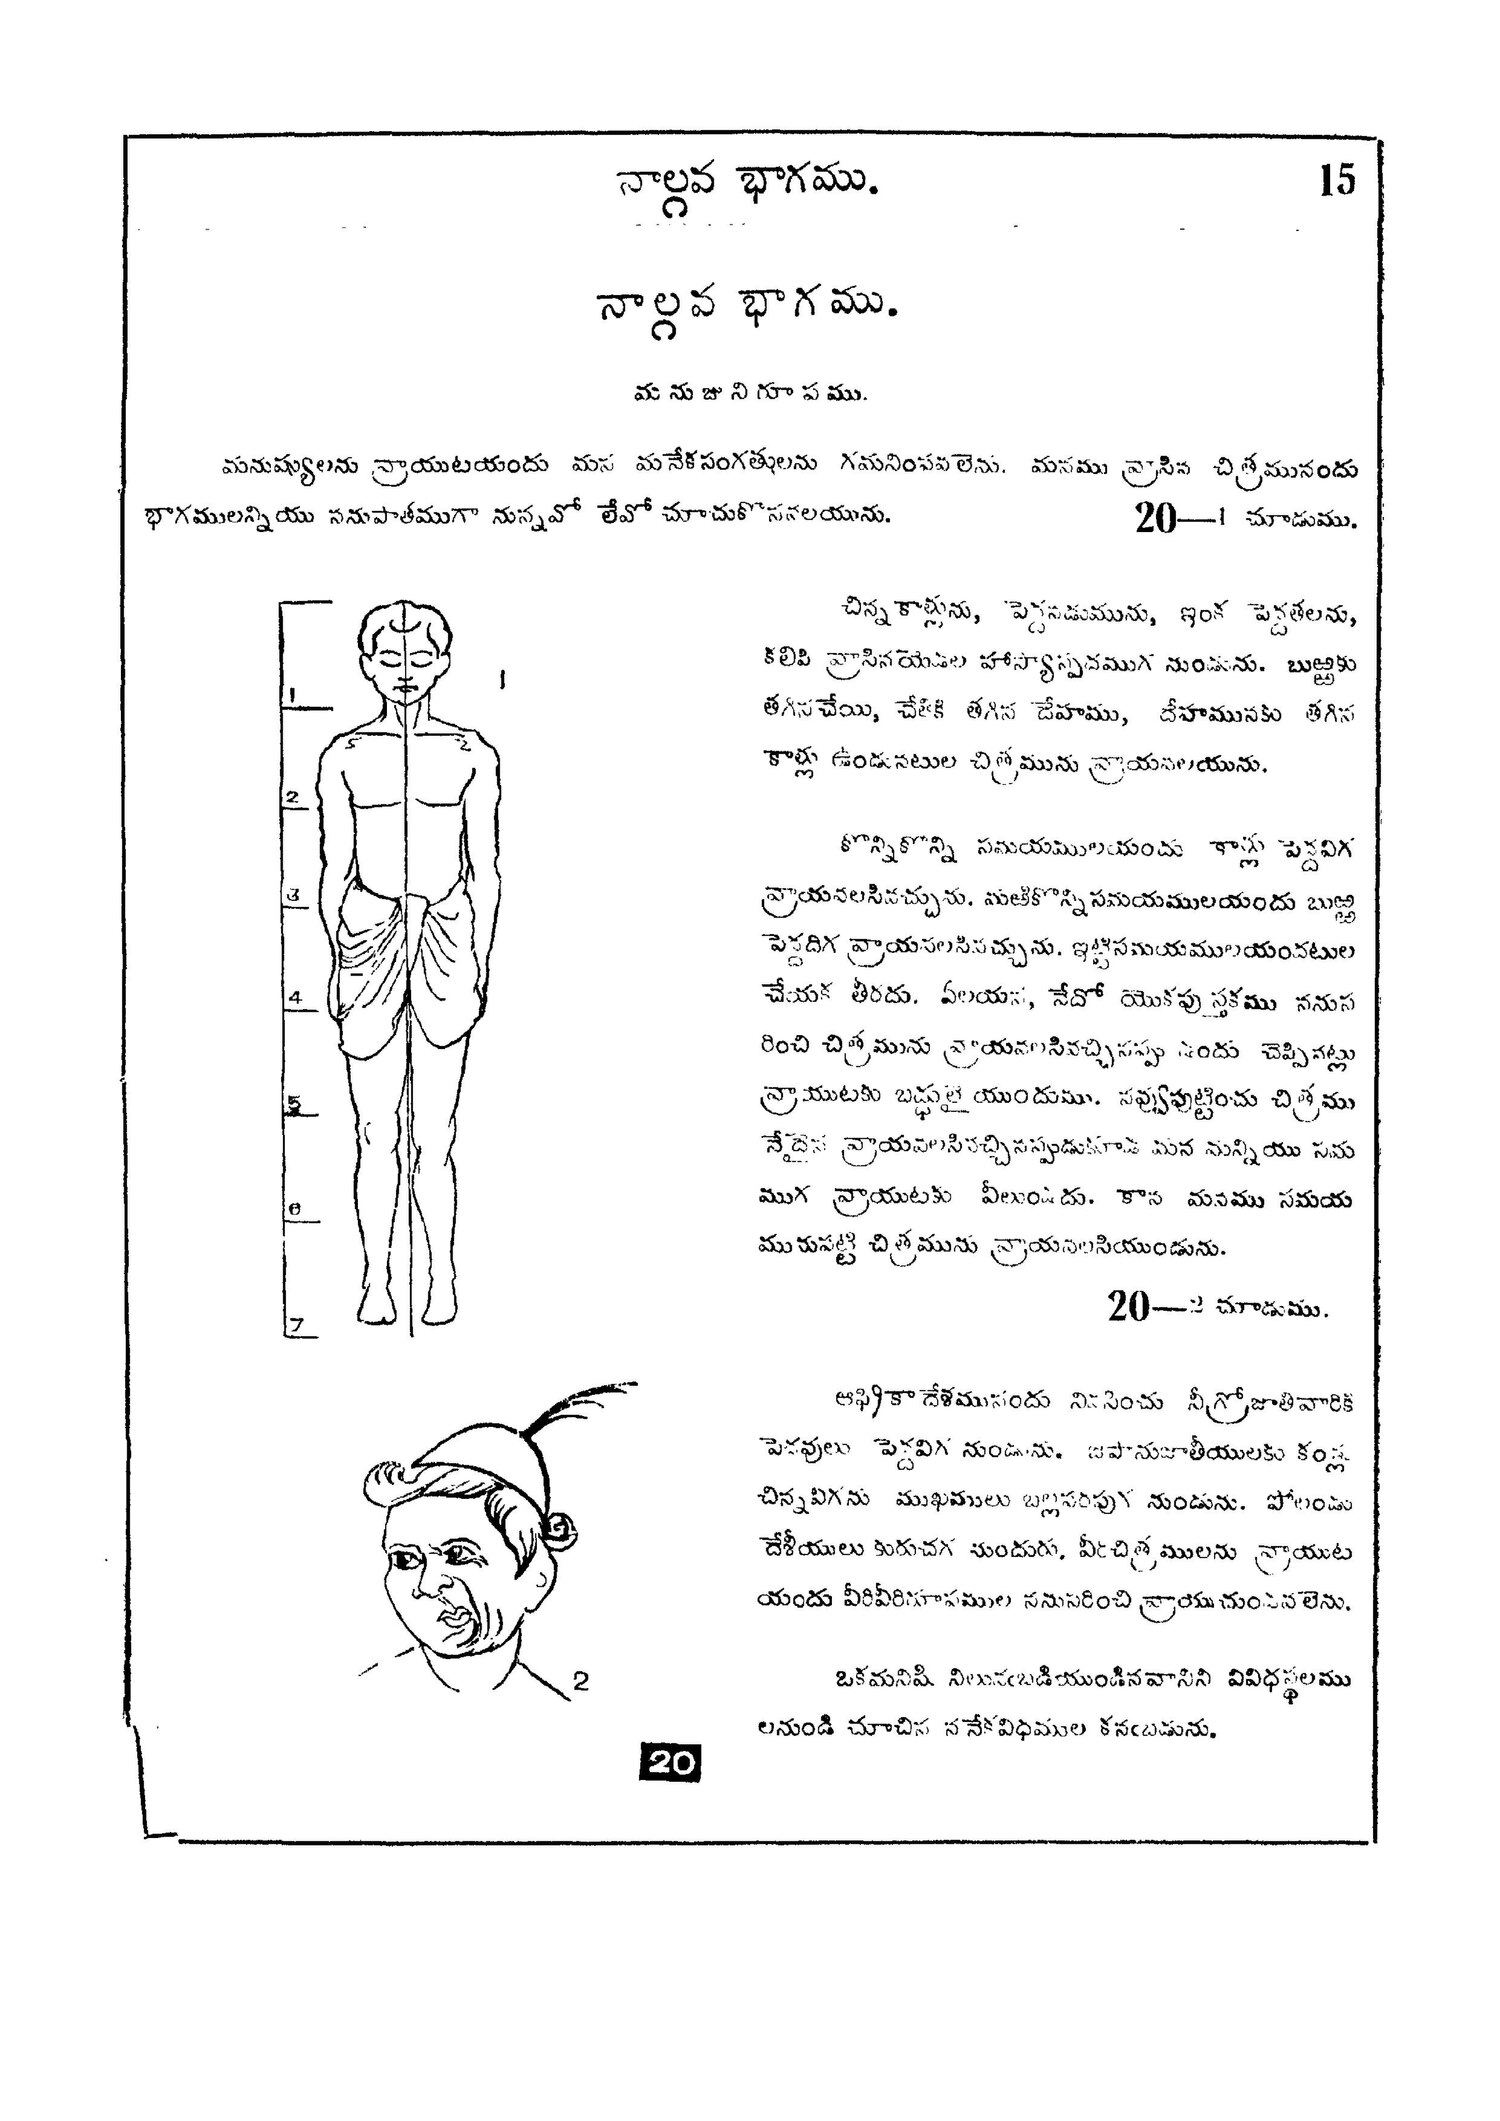
\includegraphics[width=0.6\linewidth,height=\textheight,keepaspectratio]{figures/corpus/quality_examples/complex_layout.jpg}

}

\caption{Example: complex-layout page.}

\end{figure}%

\subsection{Faded}\label{faded}

\textbf{Definition.} Pages where the text is fully present but appears
low-contrast (light ink, possibly small type) such that individual
characters are harder to read than on a Clean page. The fading is
approximately uniform across the page, not localized to one band or
edge.

\textbf{Inclusion criteria} (all must hold):

\begin{itemize}
\tightlist
\item
  Text is visibly lighter than a Clean page drawn from the same book
\item
  The low-contrast affects a substantial portion of the page (more than
  a small area)
\item
  No content is physically missing --- every character is still drawable
  if traced carefully
\end{itemize}

\textbf{Disambiguation.}

\begin{itemize}
\tightlist
\item
  If only the edges of the page are faded but the center is sharp, the
  page is assigned to Damaged (the loss is localized).
\item
  If only one horizontal band is affected, the page is Damaged.
\item
  If the page is uniformly low-contrast partly because of ink
  bleed-through from the reverse page, it remains Faded as long as the
  bleed-through does not itself obscure characters.
\end{itemize}

\textbf{OCR relevance.} This is the bucket directly addressed by the
binarization stage in Phase 2. We expect to observe a measurable CER
improvement on this bucket between the raw-OCR and preprocessed-OCR runs
in Phase 5.

\begin{figure}[H]

{\centering 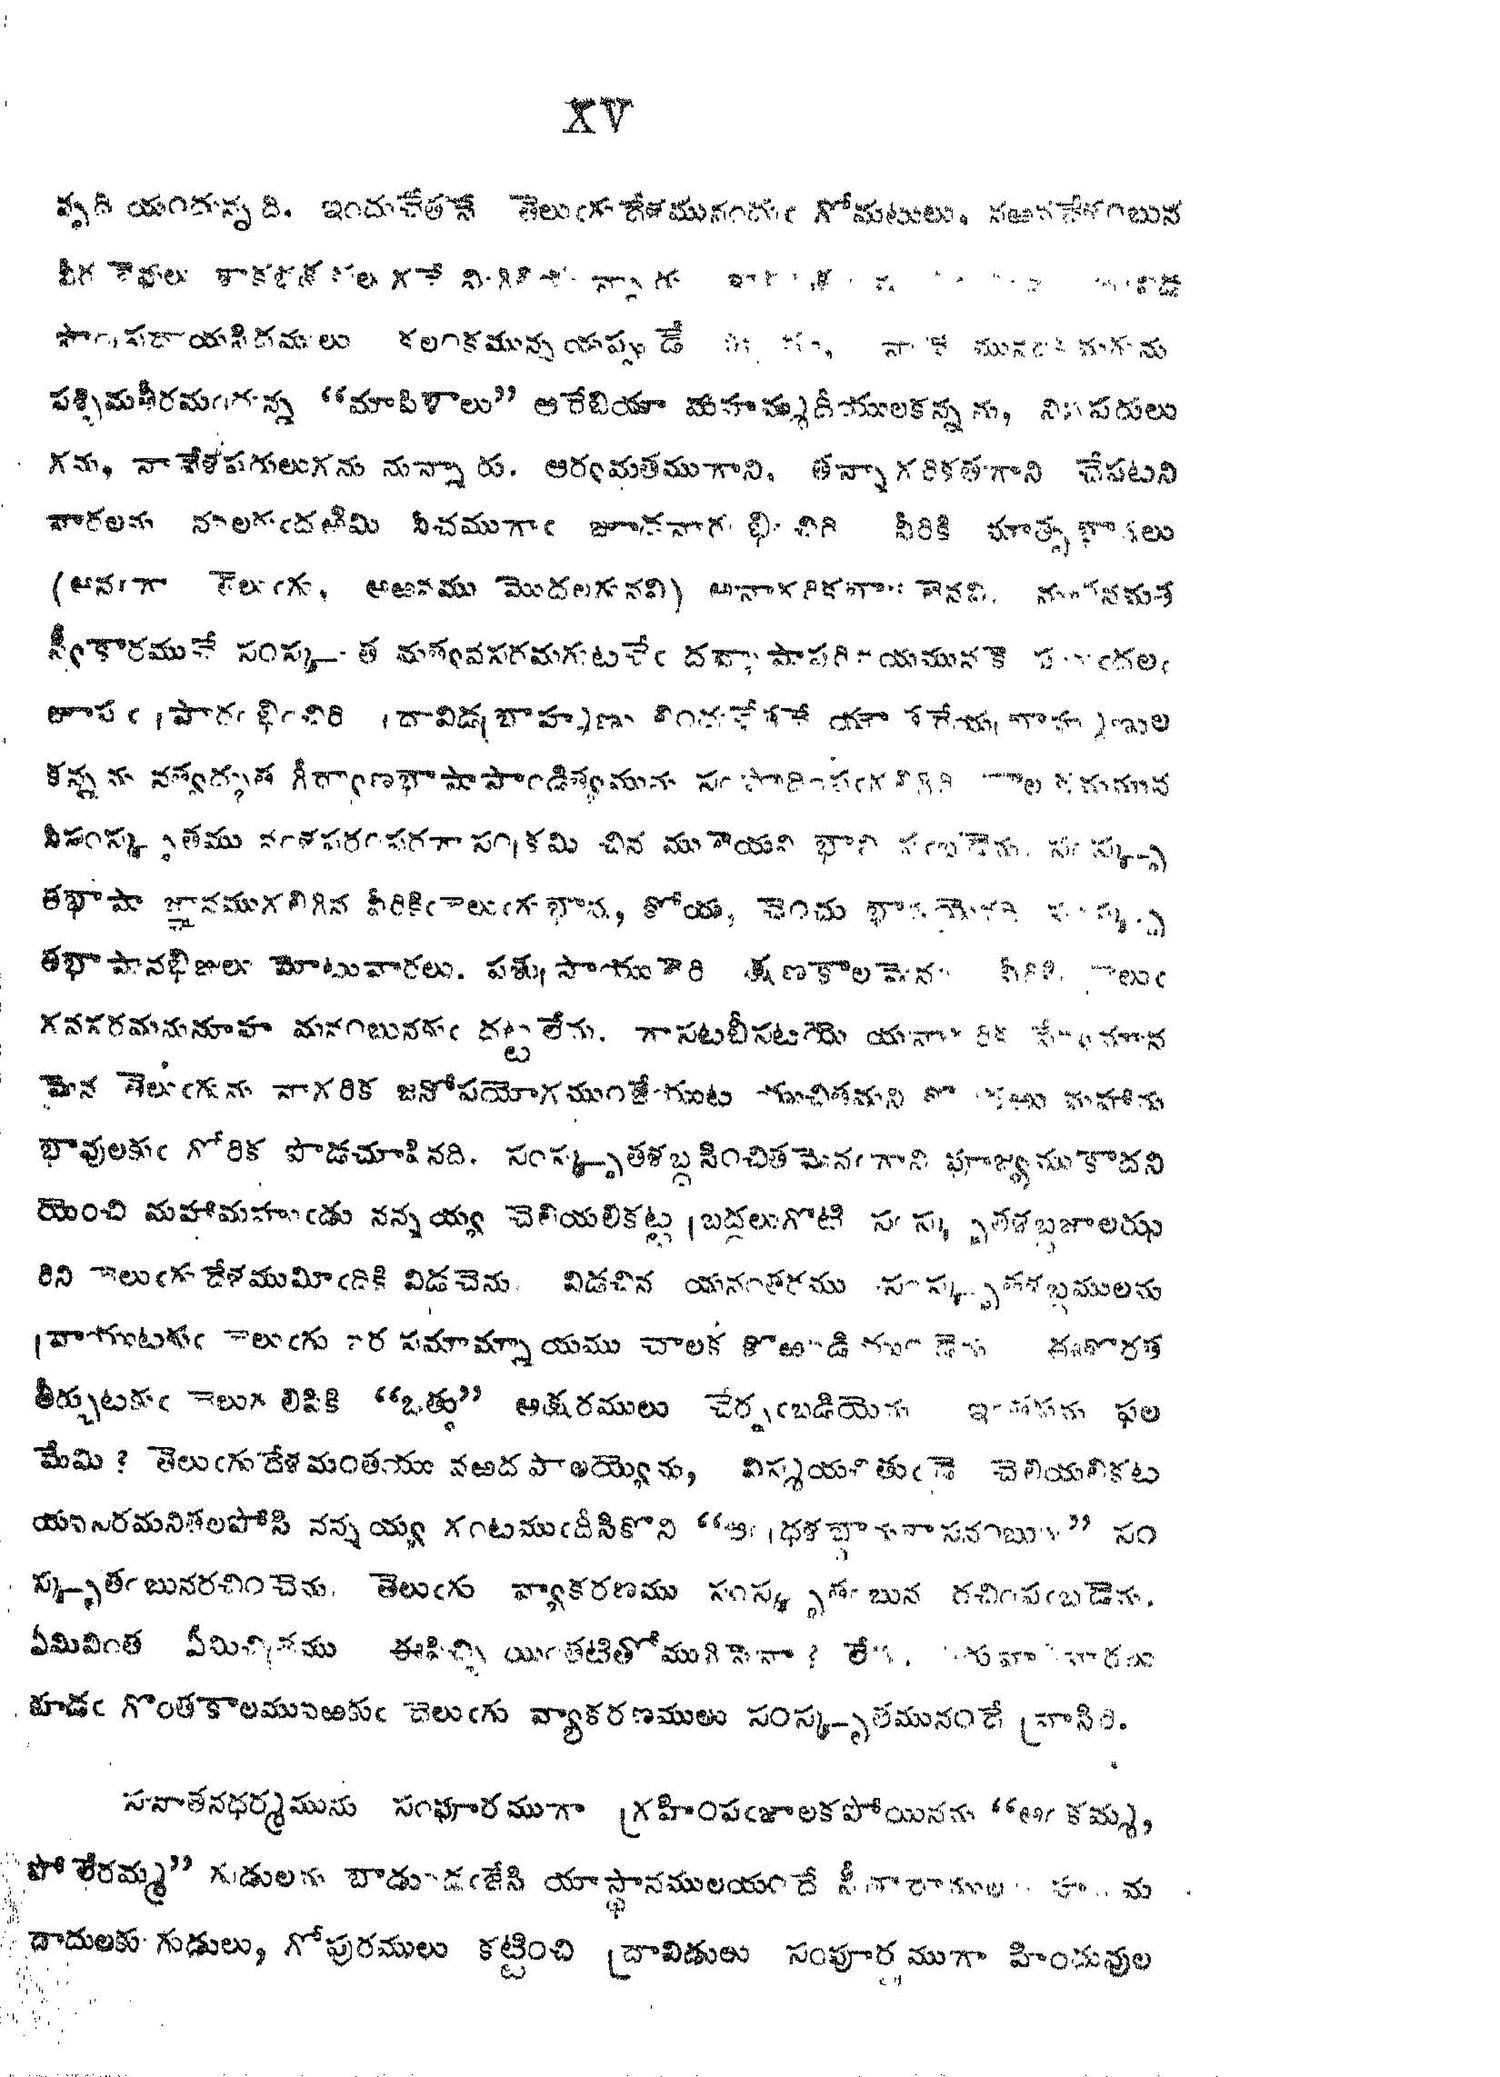
\includegraphics[width=0.6\linewidth,height=\textheight,keepaspectratio]{figures/corpus/quality_examples/faded.jpg}

}

\caption{Example: faded page.}

\end{figure}%

\subsection{Damaged / Content Loss}\label{damaged-content-loss}

\textbf{Definition.} Pages where content is physically lost or
unrecoverable due to scanning artifacts, physical damage to the source
page, or severe localized degradation. Distinguished from Faded by the
localized or discrete nature of the loss --- a Damaged page has specific
regions where information has been destroyed, not merely a uniform
reduction in contrast.

\textbf{Inclusion criteria} (any one is sufficient):

\begin{itemize}
\tightlist
\item
  White-band horizontal artifact across one or more text lines (scanning
  or photocopier artifact)
\item
  Page is visibly torn and reassembled with a discernible alignment
  offset
\item
  Significant ink smudging that obliterates words or letters
\item
  Severe edge fading where edge words are lost entirely (not merely
  lighter than the page interior)
\item
  Severe ink bleed-through where text from the reverse page is illegibly
  mixed with the front-page text such that characters cannot be reliably
  read
\item
  Any other visible damage that has removed or obscured printed content
\end{itemize}

\textbf{OCR relevance.} This bucket sets the noise floor on OCR quality.
Preprocessing cannot recover lost content. The corpus-wide CER reported
in Phase 5 is partially bounded by the fraction of pages in this bucket,
which is important context for interpreting the headline results: a 10\%
mean CER on a corpus with 15\% Damaged pages is a very different story
than a 10\% mean CER on a corpus that is entirely Clean.

\begin{figure}[H]

{\centering 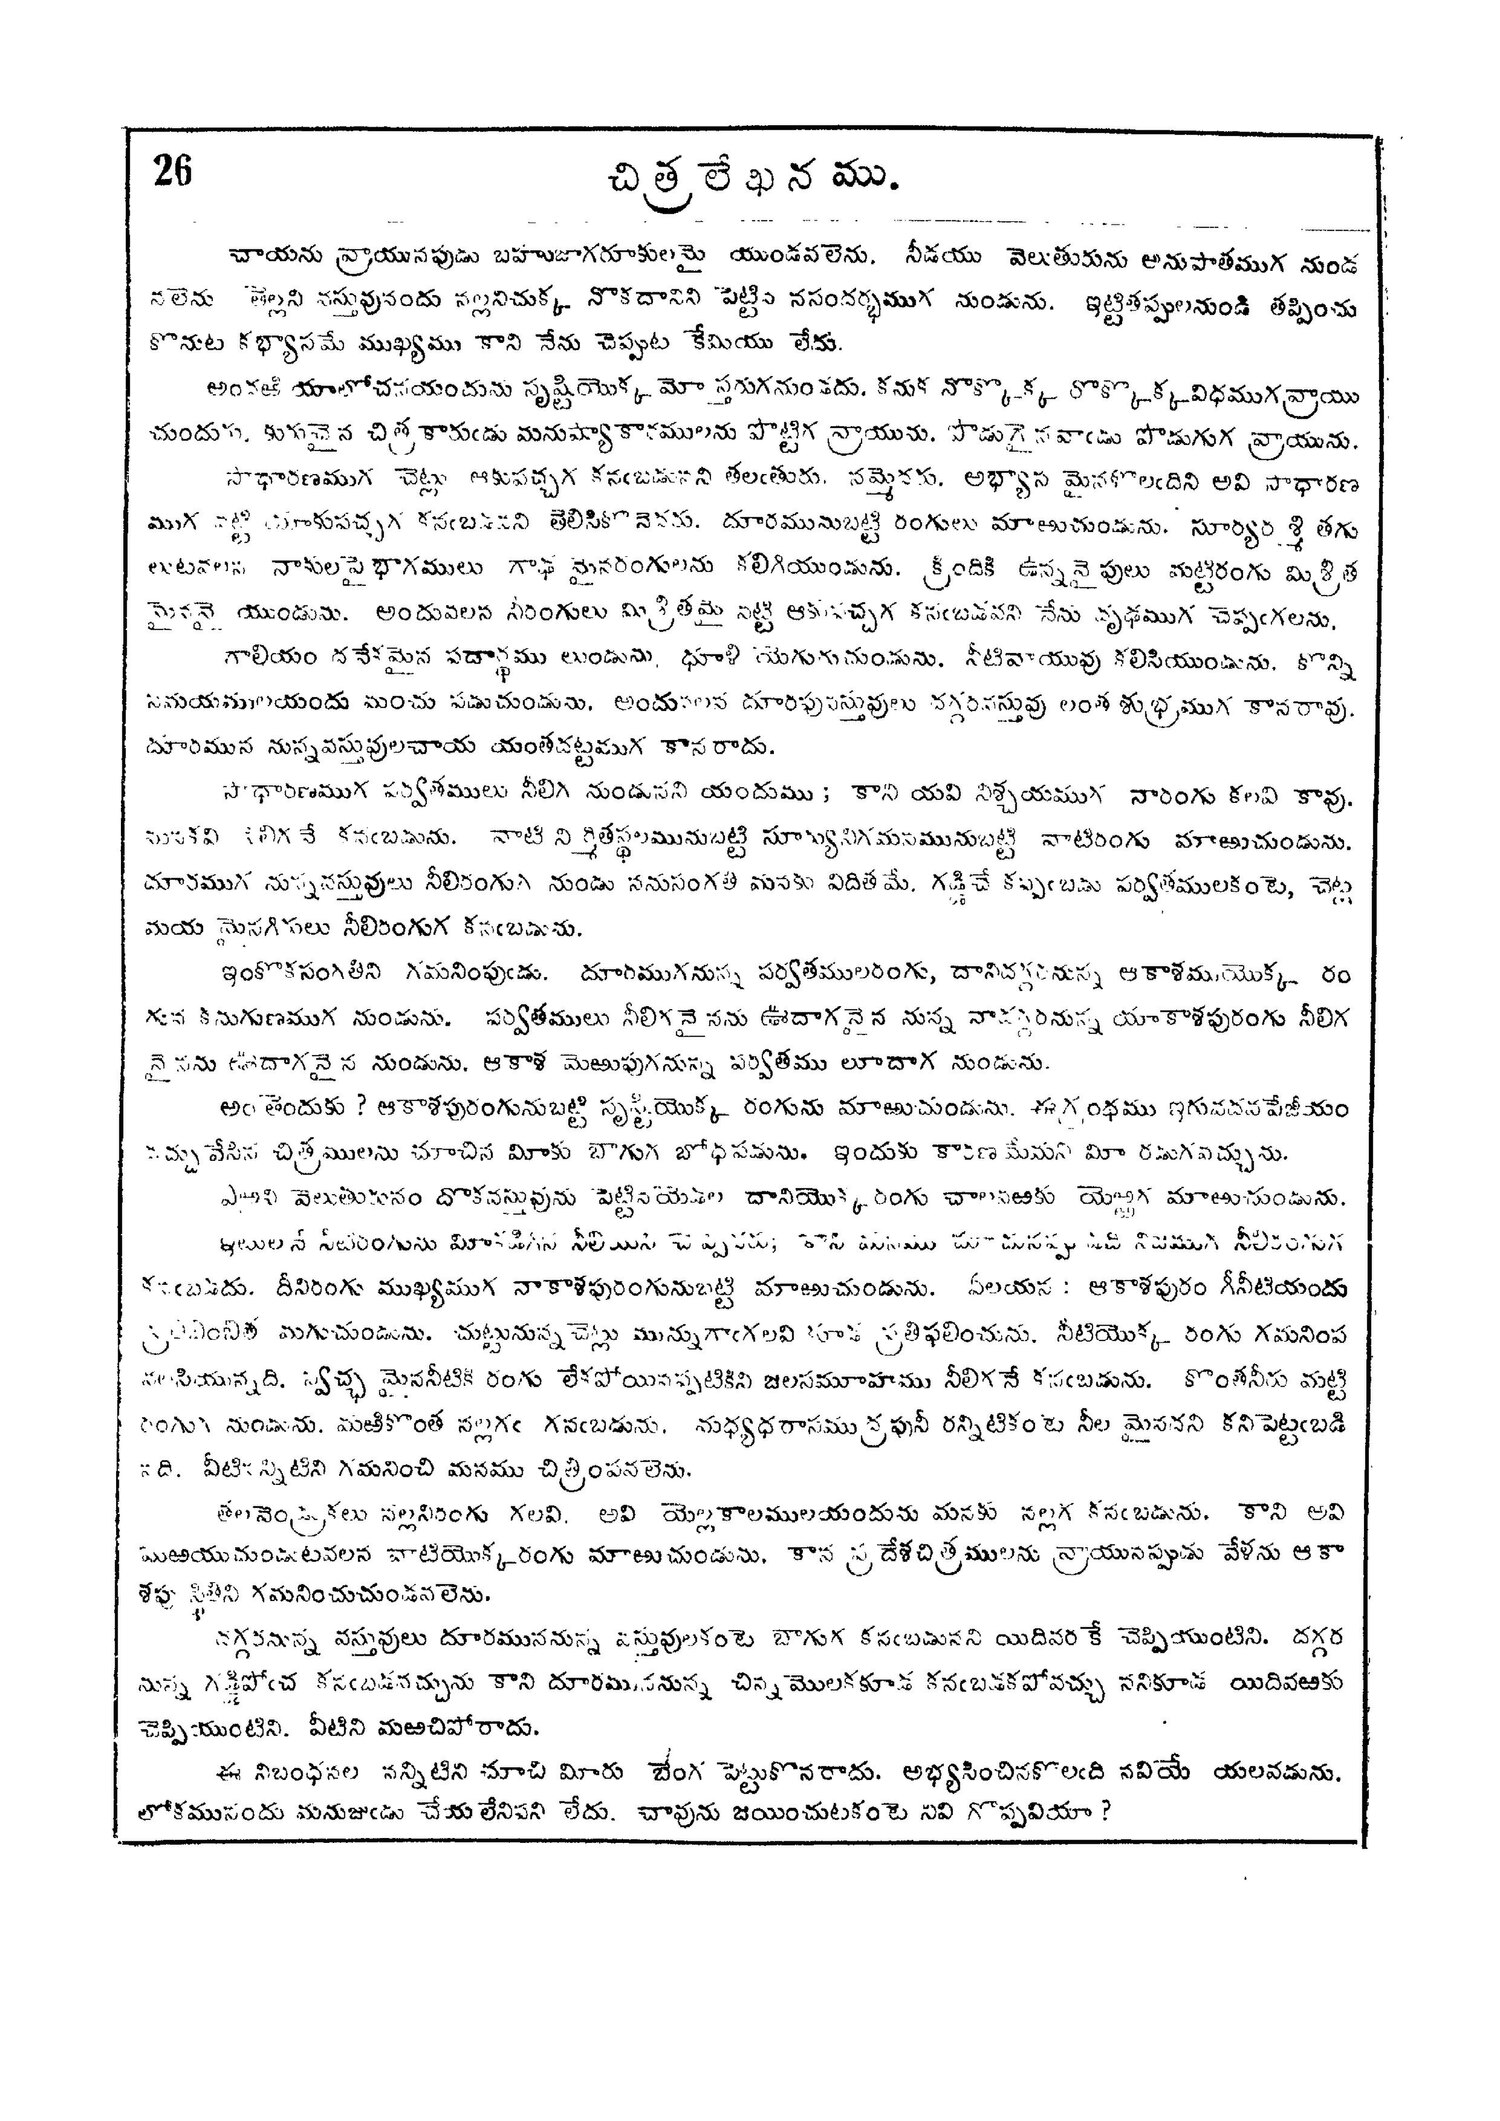
\includegraphics[width=0.6\linewidth,height=\textheight,keepaspectratio]{figures/corpus/quality_examples/damaged.jpg}

}

\caption{Example: damaged page.}

\end{figure}%

\subsection{Secondary Tag:
has\_latin\_chars}\label{secondary-tag-has_latin_chars}

Distinct from the five primary buckets, we tag each page in the
inventory CSV with a boolean \texttt{has\_latin\_chars} indicating
whether the page contains any English, Roman, or Arabic numerals or
Latin-script characters. Common cases include page numbers, numbered
verse markers (a Telugu publishing convention where individual shlokas
or verses are numbered with English digits), and citations.

This is captured as a column on the inventory CSV rather than as a
primary bucket because the feature is independent of the five quality
dimensions --- a page with English page numbers can simultaneously be
Clean, Faded, or Damaged. In Phase 5 we use this tag for an additional
analysis cut: comparing Gemini and Tesseract performance specifically on
multi-script pages, where Tesseract's \texttt{-\/-lang=tel}
configuration is expected to mishandle the Latin characters while
Gemini's vision model is expected to handle them natively.

\section{Evaluation Subset}\label{evaluation-subset}

The evaluation subset is a frozen set of 30 pages drawn stratified
across the five quality buckets --- six pages per bucket. It lives at
\texttt{data/external/eval\_subset.csv} (the page identifiers and bucket
tags) and \texttt{data/external/eval\_subset/} (the copied image and
text files). The selection script and a random seed of 42 make the draw
fully reproducible: re-running
\texttt{scripts/select\_eval\_subset.py\ -\/-seed\ 42} against the same
tagged source pool produces the identical 30-page set.

\textbf{Why stratified rather than random.} A random sample drawn from
the inventory would mirror the corpus distribution, which is heavily
Clean-dominated (approximately two-thirds of our 97-page tagged pool was
tagged Clean). On such a sample, a model that performs well on Clean
pages and poorly on Damaged pages would produce a high overall average
even if it failed on every Damaged page in the corpus. Stratified
sampling --- drawing equal numbers from each bucket --- gives us enough
statistical power per bucket to make conditional claims like ``this
preprocessing stage improves CER on Skewed pages by X\% but has no
effect on Damaged pages.'' Those conditional claims are what the
project's analysis dimension actually asks for, and a random sample
would not support them.

We deliberately accept the artificial balance as a methodological
choice. Phase 5 will report both the per-bucket CERs (computed on the
balanced eval subset) and a corpus-weighted summary CER (computed by
reweighting the per-bucket results by their estimated corpus
prevalence), so the reader sees both views.

\textbf{Why the eval subset is frozen rather than resampled per run.} If
we re-drew the evaluation pages between Phase 3 and Phase 4 --- or even
between two different OCR runs in Phase 3 --- the resulting CERs would
be incomparable, and apparent improvements between configurations would
be confounded with the random variation in page selection. Freezing the
set at the start of Phase 3, committing it to git, and using
\texttt{git\ diff} to verify it has not changed makes all per-bucket
comparisons throughout the project genuinely fair.

\textbf{Tagged source pool.} The 30-page evaluation subset is drawn from
a tagged pool of 97 pages built across two browsing batches. The first
batch (47 pages) was stratified across image-file-size quintiles and
books to spread coverage broadly. After tagging the first batch, the
Skewed bucket only contained two pages, which is too few for any
per-bucket statistical claim. A second batch (50 pages) drew randomly
from each book to top up the rare buckets; after tagging, Skewed reached
six pages and the threshold for inclusion in the stratified draw. The
full 97-page tagged pool is committed at
\texttt{data/external/quality\_tags.csv} for traceability.

\section{Challenges and Implications for
Preprocessing}\label{challenges-and-implications-for-preprocessing}

The five quality buckets are not just a corpus description; they
directly determine the preprocessing pipeline scope. Each bucket
establishes a hypothesis about which preprocessing stage is expected to
help most. Phase 5 tests those hypotheses against per-bucket CER
measurements; this section names the hypotheses explicitly.

\textbf{Skewed pages and deskew preprocessing.} Pages where the printed
content is visibly tilted in the scan frame interact badly with
classical OCR because line-segmentation algorithms typically expect
horizontal text rows. We expect the Skewed bucket to show the strongest
before-and-after CER improvement when a deskew stage is added to the
preprocessing pipeline. Deskew is therefore Stage 1 of our Phase 2
pipeline.

\textbf{Faded pages and binarization preprocessing.} Pages where the
text is uniformly low-contrast --- light ink against an off-white
background --- are harder for both classical OCR and vision LLMs because
individual characters are less visually distinct. Adaptive binarization
converts the page to a clean black-on-white representation in which
character strokes are sharper. We expect the Faded bucket to show a
strong before-and-after CER improvement when a binarization stage is
added. Binarization is therefore Stage 2 of our Phase 2 pipeline.

\textbf{Damaged pages and the noise floor.} Pages where content is
physically lost --- scanning artifacts, torn-and-reassembled pages,
severe smudging --- cannot be recovered by preprocessing because the
information is genuinely missing. We do not hypothesize any CER
improvement on Damaged pages from any preprocessing stage. Instead, we
use the Damaged bucket to characterize the noise floor on the corpus:
the lower bound on achievable CER given the dataset as shipped. A 5\%
mean CER on a corpus with 7\% Damaged pages is a very different story
than a 5\% mean CER on a fully clean corpus, and we report this context
in Phase 5.

\textbf{Complex Layout pages and the model-comparison story.} Pages
containing illustrations, multi-column text, text in frames or boxes, or
other non-uniform structure are where vision-capable LLMs are expected
to most clearly outperform classical OCR. Tesseract with
\texttt{-\/-lang=tel} and \texttt{-\/-psm\ 6} assumes a single uniform
block of text, which complex pages violate. Vision LLMs handle layout
natively and are not expected to fail on the same modes. The Complex
Layout bucket therefore provides the strongest evidence for the Phase 5
model-comparison narrative.

\textbf{Clean pages and the baseline.} Clean pages are the corpus
majority and the lower-bound case for OCR quality. The Clean bucket
establishes our best-achievable CER on the corpus given a particular
model. Strong performance on Clean is necessary but not sufficient --- a
model can score zero CER on Clean pages and still fail spectacularly on
the other four buckets, which is the entire reason for stratified
evaluation.

\section{Limitations}\label{limitations}

This characterization has explicit limitations that the reader should
keep in mind when interpreting the results in subsequent phases.

\textbf{Subset rather than full corpus.} We work with a five-book subset
(415 pages) rather than the full 13 GB upstream corpus (approximately
221 books). The subset was chosen to fit a four-day delivery schedule;
if a particular book in the full corpus contains visual conditions
absent from our five books, our taxonomy will not cover them and our
eval subset will not represent them. We mitigated this risk by drawing
the subset across file-size quintiles, which exposes the most variation
per dollar of disk space, but the risk is real and material to any claim
about ``the AlbertoChestnut corpus'' as a whole.

\textbf{JPEG compression as an unaddressed noise floor.} Every page in
the corpus is stored as a compressed JPEG. This is a publication choice
by the dataset author (likely to keep the full 13 GB tractable to host)
but it imposes a compression-artifact noise floor on the source material
that no preprocessing or OCR model in our pipeline can overcome. The
granularity that human observers notice on inspection is partly real ink
texture and partly JPEG artifact; we cannot disentangle them.

\textbf{Visual-only taxonomy by non-Telugu-reading annotators.} Neither
team member reads Telugu. Our quality taxonomy is therefore purely
visual --- we bucket pages by features observable without reading the
text. A Telugu-reading annotator might define different or additional
buckets (for example, separating ``well-typeset modern reprints'' from
``first-edition typesetting''). The buckets we use are sufficient for
OCR-relevant evaluation, but they are not the taxonomy a literary
scholar of Telugu publishing would draw.

\textbf{Ground-truth quality.} The dataset's ground-truth \texttt{.txt}
files are community-contributed and we have not independently verified
them. If the upstream ground truth has systematic errors, those errors
will appear in our reported CERs in ways we cannot easily distinguish
from OCR errors. Phase 4's LLM validation framework partially
stress-tests this concern by independently scoring OCR output for
plausibility, but the reader should not interpret reported CER values as
character-perfect ground truth.

\textbf{Per-bucket sample size of six.} Six pages per bucket gives just
enough statistical power to identify large effects between
configurations (for example, ``deskew preprocessing roughly halves CER
on Skewed pages''). It is not enough to identify subtle differences.
Phase 5 reports per-bucket effect sizes and discusses statistical
significance honestly.

\section{References}\label{references}

\begin{itemize}
\tightlist
\item
  AlbertoChestnut. \emph{Telugu OCR Dataset.} HuggingFace Hub, 2026.
  \url{https://huggingface.co/datasets/AlbertoChestnut/telugu-ocr}.
  Pinned revision: \texttt{f2bd895b4932b648174a8f47066f4166469933a0}.
  Accessed June 2026.
\item
  Morris, A. C., Maier, V., and Green, P. \emph{From WER and RIL to MER
  and WIL: improved evaluation measures for connected speech
  recognition.} INTERSPEECH 2004. (Background on word- and
  character-error-rate metrics used in Phase 4.)
\item
  Allaire, J. J., et al.~\emph{Quarto.} \url{https://quarto.org/}.
  Documentation accessed June 2026.
\item
  Smith, R. \emph{An Overview of the Tesseract OCR Engine.} In
  Proceedings of the Ninth International Conference on Document Analysis
  and Recognition, 2007.
\item
  Google. \emph{Gemini API documentation.}
  \url{https://ai.google.dev/gemini-api/docs}. Accessed June 2026.
\end{itemize}

\begin{tcolorbox}[enhanced jigsaw, arc=.35mm, bottomrule=.15mm, breakable, colback=white, colframe=quarto-callout-note-color-frame, left=2mm, leftrule=.75mm, opacityback=0, rightrule=.15mm, toprule=.15mm]
\begin{minipage}[t]{5.5mm}
\textcolor{quarto-callout-note-color}{\faInfo}
\end{minipage}%
\begin{minipage}[t]{\textwidth - 5.5mm}

\end{minipage}%
\end{tcolorbox}




\end{document}
